\documentclass[a4paper,10.5pt,uplatex]{jsarticle}
%--脚注の設定
\usepackage{natbib}
\bibpunct[, ]{(}{)}{;}{and}{}{,} %本文での引用の体裁はここで整えられるみたい
\bibliographystyle{apsr2006Edited} 
\usepackage{amsmath}
%--余白の設定
\usepackage[truedimen,margin=20truemm]{geometry}
%--図の設定
\usepackage[dvipdfmx]{graphicx,xcolor} % PDFの利用もOKに
\graphicspath{{./figures/}} %To add paths relative to the latexfile invoking the command
  %\usepackage[dvips]{graphicx}
%--行間の設定
\usepackage{setspace} 
\setstretch{1.13} % ページ全体の行間を設定
%--コードの設定
\usepackage{listings}
\usepackage{color}
\definecolor{dkgreen}{rgb}{0,0.6,0}
\definecolor{mygray}{rgb}{0.5,0.5,0.5}
\definecolor{mauve}{rgb}{0.58,0,0.82}

\definecolor{codegreen}{rgb}{0,0.6,0}
\definecolor{codegray}{rgb}{0.5,0.5,0.5}
\definecolor{codepurple}{rgb}{0.58,0,0.82}
\definecolor{backgroundcolour}{rgb}{0.95,0.95,0.95}

\usepackage{inconsolata} % Font for code
\lstset{ %
  language= {Python}, %ここを含めなければ、変に太字になったりしない
  aboveskip=2.5mm,
  belowskip=4.5mm,
  showstringspaces=false,
  columns=flexible,
  keepspaces=true,
  numbers=left,                    
  numbersep=5pt,    
  basicstyle={\small\fontfamily{zi4}\selectfont},
  commentstyle={\small\fontfamily{zi4}\selectfont},
  breaklines=true,
  breakatwhitespace=true,
  tabsize=3,
  frame=single, % lines or delete this line
  backgroundcolor=\color{backgroundcolour},   
  commentstyle=\color{codegreen},
  keywordstyle=\color{magenta},
  numberstyle=\tiny\color{codegray},
  stringstyle=\color{codepurple},
  xleftmargin = 1.1cm,
  framexleftmargin = 1em
}
\usepackage{xcolor}
\usepackage{framed}
\colorlet{shadecolor}{green!8}
%--リンクの埋め込みを可能にする  \href{ **URL** }{表示テキスト}
\usepackage[dvipdfmx]{hyperref}
\usepackage{courier}
\usepackage{here}
%--日本語環境用の設定を追加
% \usepackage[english]{babel} % まとめて英語化できる
 % \addto\captionsenglish{\renewcommand{\figurename}{Figure }} %jsarticleでFigureにスペースが入らないのを調整
 % \addto\captionsenglish{\renewcommand{\tablename}{Table }}
 \renewcommand{\lstlistingname}{Code}
\renewcommand{\refname}{参考文献}
\renewcommand{\abstractname}{要約}
\usepackage{multirow}
\usepackage{placeins}
%--数学用のフォント
\usepackage{amsmath} 
\usepackage{amssymb}
\usepackage{amsfonts}
%--セクションのフォント
\renewcommand{\headfont}{\bfseries}
% Tikz
\usepackage{tikz}
\usepackage{bayesnet}
%-----------------
\begin{document}

\title{}
\author{NAME\thanks{AFFILIATION}}
\date{20**/**/**}
\maketitle
%\begin{abstract}
%\end{abstract}

\begin{figure}[!h]
\centering
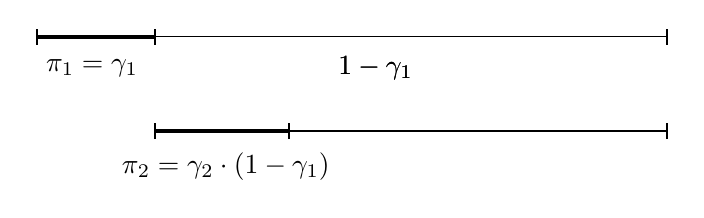
\begin{tikzpicture}
 
  % Level 1
  \draw [line width=0.2mm](-4,0)--(4,0);
  \draw [line width=0.5mm](-4,0)--(-2.5,0);
  \draw [thick] (-4,-.1) node[below]{} -- (-4,0.1);
  \draw [thick] (4,-.1) node[below]{} -- (4,0.1);
  \draw [thick] (-2.5,-.1) node[below]{} -- (-2.5,0.1);
  \node at (-3.3, -0.4) {$\pi_1 = \gamma_1$};
  \node at (.3, -0.4) {$1 - \gamma_1$};
  
  % Level 2
  \draw [line width=0.2mm](-2.5,-1.2)--(4,-1.2);
  \draw [line width=0.5mm](-2.5,-1.2)--(-.8,-1.2);
  \draw [thick] (-2.5,-1.3) node[below]{} -- (-2.5,-1.1);
  \draw [thick] (4,-1.3) node[below]{} -- (4,-1.1);
  \draw [thick] (-0.8,-1.3) node[below]{} -- (-0.8,-1.1);
  \node at (-1.6, -1.65) {$\pi_2 = \gamma_2 \cdot (1 - \gamma_1)$};
  \node at (.3, -0.4) {$1 - \gamma_1$};
 
\end{tikzpicture}
\end{figure}

\begin{figure}[!h]
\centering
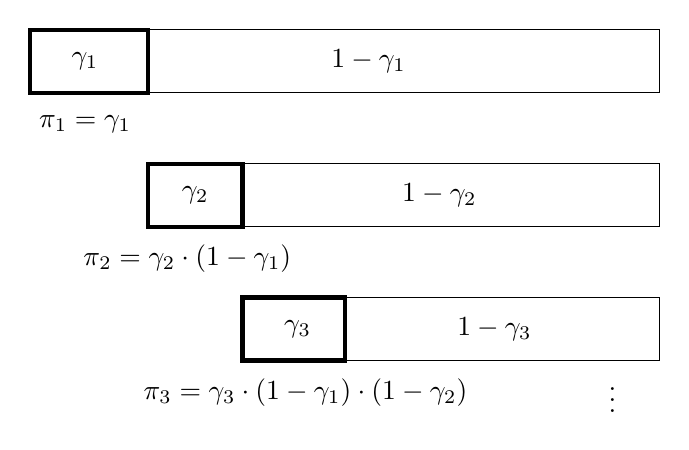
\begin{tikzpicture}
 
  % Level 1
  \draw [] (-4,0) rectangle (4,0.8);
  \draw [ultra thick] (-4,0) rectangle (-2.5,0.8);
  \node at (-3.3, 0.4) {$\gamma_1$};
  \node at (-3.3, -0.4) {$\pi_1 = \gamma_1$};
  \node at (.3, 0.4) {$1 - \gamma_1$};
  
  % Level 2
  \draw [] (-2.5,-1.7) rectangle (4,-0.9);
  \draw [ultra thick] (-2.5,-1.7) rectangle (-1.3,-0.9);
  \node at (-1.9, -1.3) {$\gamma_2$};
  \node at (1.2, -1.3) {$1 - \gamma_2$};
  \node at (-2, -2.1) {$\pi_2 = \gamma_2 \cdot (1 - \gamma_1)$};

  % Level 3
  \draw [] (-1.3,-3.4) rectangle (4,-2.6);
  \draw [ultra thick] (-1.3,-3.4) rectangle (0,-2.6);
  \node at (-0.6, -3) {$\gamma_3$};
  \node at (1.9, -3) {$1 - \gamma_3$};
  \node at (-0.5, -3.8) {$\pi_3 = \gamma_3 \cdot (1 - \gamma_1) \cdot (1 - \gamma_2)$};
  \node at (3.4, -3.8) {$\vdots$};
 
\end{tikzpicture}
\end{figure}

\begin{figure}[!htb]
\centering
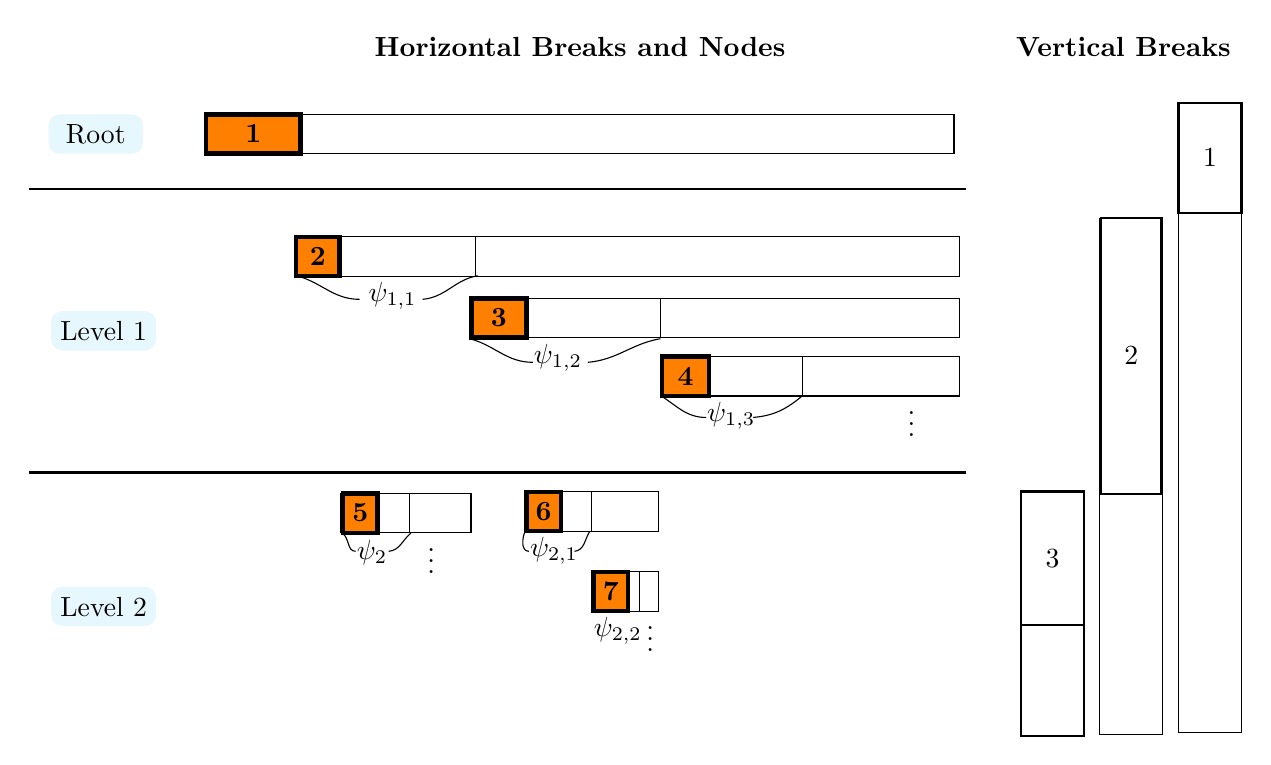
\begin{tikzpicture}
  % Text
  \node (RootText) at (-5,1.1) [minimum width=1.2cm, minimum height=0.5cm, ] {\textbf{Horizontal Breaks and Nodes}}; 
  \node (RootText) at (1.9,1.1) [minimum width=1.2cm, minimum height=0.5cm, ] {\textbf{Vertical Breaks}}; 

  % Level 1 Horizontal
  \node (Level1H) at (-5,0) [draw,minimum width=9.5cm, minimum height=0.5cm] {}; 
  \node (Level1HStop) at ([shift={(-4.15,0)}]Level1H) [draw, ultra thick, minimum width=1.2cm, minimum height=0.5cm, fill=orange] {\textbf{1}};
  \draw [line width=0.3mm](-12,-0.7)--(-0.1,-0.7);
  \node (RootText) at ([shift={(-6.15,0)}]Level1H) [minimum width=1.2cm, minimum height=0.5cm, fill=cyan!10, rounded corners] {Root}; 

  % Level 1 Vertical
  \node (Level1V) at ([shift={(8,-3.6)}]Level1H) [draw,minimum width=0.8cm, minimum height=8cm] {};
  \node (Level1VStop) at ([shift={(0,3.295)}]Level1V) [draw, thick, minimum width=0.8cm, minimum height=1.4cm] {1};

  % Level 2 Horizontal
  \node (Level2H) at ([shift={(0.62,-1.3)}]Level1H) [draw,minimum width=8.4cm, minimum height=0.5cm, below] {};
  \node at ([shift={(-3,-0.5)}]Level2H) {$\psi_{1,1}$};
  \draw[] (-8.6,-1.8) to [out=-15,in=180] (-7.8,-2.1);
  \draw[] (-7.0,-2.1) to [out=5,in=190] (-6.3,-1.8);
  \node (Level2HStop) at ([shift={(-3.95,0)}]Level2H) [draw, ultra thick, minimum width=0.55cm, minimum height=0.5cm, fill=orange] {\textbf{2}};
  \node (Level2HLine1) at ([shift={(-3.1,0)}]Level2H) [draw, minimum width=2.3cm, minimum height=0.5cm] {};

  \node (Level2H2) at ([shift={(1.1,-0.78)}]Level2H) [draw,minimum width=6.2cm, minimum height=0.5cm] {};
  \node at ([shift={(-2,-0.5)}]Level2H2) {$\psi_{1,2}$};
  \draw[] (-6.4,-2.6) to [out=-15,in=180] (-5.6,-2.9);
  \draw[] (-4.9,-2.9) to [out=5,in=190] (-3.98,-2.6);
  \node (Level2HStop2) at ([shift={(-2.75,0)}]Level2H2) [draw, ultra thick, minimum width=0.7cm, minimum height=0.5cm, fill=orange] {\textbf{3}};
  \node (Level2HLine2) at ([shift={(-1.9,0)}]Level2H2) [draw, minimum width=2.4cm, minimum height=0.5cm] {};

  \node (Level2H3) at ([shift={(2.3,-1.52)}]Level2H) [draw,minimum width=3.8cm, minimum height=0.5cm] {};
  \node at ([shift={(-1,-0.5)}]Level2H3) {$\psi_{1,3}$};
  \draw[] (-3.98,-3.32) to [out=-32,in=180] (-3.4,-3.6);
  \draw[] (-2.8,-3.6) to [out=5,in=220] (-2.17,-3.32);
  \node (Level2HStop3) at ([shift={(-1.58,0)}]Level2H3) [draw, ultra thick, minimum width=0.6cm, minimum height=0.5cm, fill=orange] {\textbf{4}};
  \node (Level2HLine3) at ([shift={(-0.99,0)}]Level2H3) [draw, minimum width=1.8cm, minimum height=0.5cm] {};
  \node at  ([shift={(1.29,-0.5)}]Level2H3) {$\vdots$};

  \node (Level1Text) at ([shift={(0.1,-2.5)}]RootText) [minimum width=1.2cm, minimum height=0.5cm, fill=cyan!10, rounded corners] {Level 1};
  \draw [line width=0.3mm](-12,-4.3)--(-0.1,-4.3);

  % Level 2 Vertical
  \node (Level2V) at ([shift={(-1,-0.75)}]Level1V) [draw, minimum width=0.8cm, minimum height=6.55cm] {};
  \node (Level2VStop) at ([shift={(0,1.53)}]Level2V) [draw, thick, minimum width=0.77cm, minimum height=3.5cm] {2};

  % Level 3 Horizontal
  \node (Level3H1) at ([shift={(-2.83,-3.0)}]Level2H) [draw,minimum width=1.65cm, minimum height=0.5cm, below] {};
  \node at ([shift={(-0.43,-0.5)}]Level3H1) {$\psi_{2}$};
  \draw[] (-8.02,-5.07) to [out=-32,in=180] (-7.85,-5.3);
  \draw[] (-7.43,-5.3) to [out=5,in=220] (-7.15,-5.07);
  \node (Level3HStop1) at ([shift={(-0.58,0)}]Level3H1) [draw, ultra thick, minimum width=0.2cm, minimum height=0.5cm, fill=orange] {\textbf{5}};
  \node (Level3HLine1) at ([shift={(-0.39,0)}]Level3H1) [draw, minimum width=0.86cm, minimum height=0.5cm] {};
  \node at  ([shift={(0.32,-0.5)}]Level3H1) {$\vdots$};

  \node (Level3H) at ([shift={(-1.57,-2.2)}]Level2H2) [draw,minimum width=1.7cm, minimum height=0.5cm, below] {};
  \node at ([shift={(-0.48,-0.5)}]Level3H) {$\psi_{2,1}$};
  \draw[] (-5.70,-5.05) to [out=-112,in=180] (-5.65,-5.3);
  \draw[] (-5.07,-5.3) to [out=5,in=240] (-4.88,-5.05);
  \node (Level3HStop2) at ([shift={(-0.612,0)}]Level3H) [draw, ultra thick, minimum width=0.2cm, minimum height=0.5cm, fill=orange] {\textbf{6}};
  \node (Level3HLine2) at ([shift={(-0.402,0)}]Level3H) [draw, minimum width=0.8cm, minimum height=0.5cm] {};

  \node (Level3H1) at ([shift={(0.45,-0.76)}]Level3H) [draw,minimum width=0.80cm, minimum height=0.5cm, below] {};
  \node at ([shift={(-0.12,-0.5)}]Level3H1) {$\psi_{2,2}$};
  \node (Level3HStop3) at ([shift={(-0.209,0)}]Level3H1) [draw, ultra thick, minimum width=0.2cm, minimum height=0.5cm, fill=orange] {\textbf{7}};
  \node (Level3HLine3) at ([shift={(-0.14,0)}]Level3H1) [draw, minimum width=0.6cm, minimum height=0.5cm] {};
  \node at  ([shift={(0.29,-0.5)}]Level3H1) {$\vdots$};

  \node (Level2Text) at ([shift={(0,-3.5)}]Level1Text) [minimum width=1.2cm, minimum height=0.5cm, fill=cyan!10, rounded corners] {Level 2};

  % Level 3 Vertical
  \node (Level3V) at ([shift={(-1,-1.75)}]Level2V) [draw, minimum width=0.8cm, minimum height=3.09cm] {};
  \node (Level3VStop) at ([shift={(0,0.71)}]Level3V) [draw, thick, minimum width=0.8cm, minimum height=1.7cm] {3};
\end{tikzpicture}
\caption{Tree-Structured Stick Breaking Process}
\label{fig:TSSBfromSBP}
\end{figure}


\begin{figure}[!htb]
\centering
\begin{tikzpicture}
  % Nodes
  % parameters and data
  \node[latent]           (1)    {\textbf{1}}; %
  \node[latent, below= of 1]  (3) {\textbf{3}};
  \node[latent, left= of 3]  (2) {\textbf{2}};
  \node[latent, right= of 3]  (4) {\textbf{4}};
  \node[latent, below= of 2]  (5) {\textbf{5}};
  \node[latent, below= of 3, xshift=-0.5cm]  (6) {\textbf{6}};
  \node[latent, below= of 3, xshift=0.5cm]  (7) {\textbf{7}};
  % edges
  \edge[-]{1}{2};
   \edge[-]{1}{3};
   \edge[-]{1}{4};
   \edge[-]{2}{5};
   \edge[-]{3}{6};
   \edge[-]{3}{7};
\end{tikzpicture}
\caption{Nodes in TSSB}
\end{figure}

\begin{alignat}{2}
  \pi_7 &= \nu_7 \cdot \psi_7  & {\rm Stop\ at\ Node\ 7}\\
        &\ \ \times (1 - \psi_6)  & {\rm Pass\ Node\ 6}\\
        &\ \ \times (1 - \nu_3) \cdot \psi_3 \cdot (1 - \psi_2)   &{\rm Pass\ Node\ 3}\\
        &\ \ \times (1 - \nu_1) & {\rm Pass\ Node\ 1}
\end{alignat}

%\bibliography{ref}
\end{document}
